\documentclass[11pt,twoside,a4paper,openright]{report}
%%%%%%%%%%%%%%%%%%%%%%%%%%%%%%%%%%%%%%%%%%%%%%%%
% Language, Encoding and Fonts
% http://en.wikibooks.org/wiki/LaTeX/Internationalization
%%%%%%%%%%%%%%%%%%%%%%%%%%%%%%%%%%%%%%%%%%%%%%%%
% Select encoding of your inputs. Depends on
% your operating system and its default input
% encoding. Typically, you should use
%   Linux  : utf8 (most modern Linux distributions)
%            latin1 
%   Windows: ansinew
%            latin1 (works in most cases)
%   Mac    : applemac
% Notice that you can manually change the input
% encoding of your files by selecting "save as"
% an select the desired input encoding. 
\usepackage[utf8]{inputenc}
% Make latex understand and use the typographic
% rules of the language used in the document.
\usepackage[danish,english]{babel}
% Use the palatino font
\frenchspacing
\usepackage[sc]{mathpazo}
\linespread{1.05}         % Palatino needs more leading (space between lines)
% Choose the font encoding
\usepackage[T1]{fontenc}
%Symbol dictionary package(used for tick symbol)
\usepackage{bbding}

%%%%%%%%%%%%%%%%%%%%%%%%%%%%%%%%%%%%%%%%%%%%%%%%
% Graphics and Tables
% http://en.wikibooks.org/wiki/LaTeX/Importing_Graphics
% http://en.wikibooks.org/wiki/LaTeX/Tables
% http://en.wikibooks.org/wiki/LaTeX/Colors
%%%%%%%%%%%%%%%%%%%%%%%%%%%%%%%%%%%%%%%%%%%%%%%%
% load a colour package
\usepackage{xcolor}
\definecolor{aaublue}{RGB}{33,26,82}% dark blue
% The standard graphics inclusion package
\usepackage{graphicx}
% Set up how figure and table captions are displayed
\usepackage{subcaption}
\usepackage{caption}
\captionsetup{%
  font=footnotesize,% set font size to footnotesize
  labelfont=bf % bold label (e.g., Figure 3.2) font
}
% Make the standard latex tables look so much better
\usepackage{array,booktabs,tabularx,multirow}
% Enable the use of frames around, e.g., theorems
% The framed package is used in the example environment
\usepackage{framed}

% Adds support for full page background picture
\usepackage[contents={},color=gray]{background}
%\usepackage[contents=draft,color=gray]{background}

%%%%%%%%%%%%%%%%%%%%%%%%%%%%%%%%%%%%%%%%%%%%%%%%
% Mathematics
% http://en.wikibooks.org/wiki/LaTeX/Mathematics
%%%%%%%%%%%%%%%%%%%%%%%%%%%%%%%%%%%%%%%%%%%%%%%%
% Defines new environments such as equation,
% align and split 
\usepackage{mathtools}
% Adds new math symbols
\usepackage{amssymb}
% Use theorems in your document
% The ntheorem package is also used for the example environment
% When using thmmarks, amsmath must be an option as well. Otherwise \eqref doesn't work anymore.
\usepackage[framed,amsmath,thmmarks]{ntheorem}

%%%%%%%%%%%%%%%%%%%%%%%%%%%%%%%%%%%%%%%%%%%%%%%%
% Page Layout
% http://en.wikibooks.org/wiki/LaTeX/Page_Layout
%%%%%%%%%%%%%%%%%%%%%%%%%%%%%%%%%%%%%%%%%%%%%%%%
% Change margins, papersize, etc of the document
\usepackage[
  inner=28mm,% left margin on an odd page
  outer=41mm,% right margin on an odd page
  headheight=13.6pt,
  bottom=39mm
  ]{geometry}
% Modify how \chapter, \section, etc. look
% The titlesec package is very configureable
\usepackage{titlesec}
\titleformat{\chapter}[display]{\normalfont\huge\bfseries}{\chaptertitlename\ \thechapter}{20pt}{\Huge}
\titleformat*{\section}{\normalfont\Large\bfseries}
\titleformat*{\subsection}{\normalfont\large\bfseries}
\titleformat*{\subsubsection}{\normalfont\normalsize\bfseries}
%\titleformat*{\paragraph}{\normalfont\normalsize\bfseries}
%\titleformat*{\subparagraph}{\normalfont\normalsize\bfseries}

% Clear empty pages between chapters
\let\origdoublepage\cleardoublepage
\newcommand{\clearemptydoublepage}{%
  \clearpage
  {\pagestyle{empty}\origdoublepage}%
}
\let\cleardoublepage\clearemptydoublepage

% Change the headers and footers
\usepackage{fancyhdr}
\pagestyle{fancy}
\fancyhf{} %delete everything
\renewcommand{\headrulewidth}{0pt} %remove the horizontal line in the header
\fancyhead[RE]{\small\nouppercase\leftmark} %even page - chapter title
\fancyhead[LO]{\small\nouppercase\rightmark} %uneven page - section title
\fancyhead[LE,RO]{\thepage \hspace{1pt} of \pageref{LastPage}} %page number on all pages
% Do not stretch the content of a page. Instead,
% insert white space at the bottom of the page
\raggedbottom
% Enable arithmetics with length. Useful when
% typesetting the layout.
\usepackage{calc}

%%%%%%%%%%%%%%%%%%%%%%%%%%%%%%%%%%%%%%%%%%%%%%%%
% Bibliography
% http://en.wikibooks.org/wiki/LaTeX/Bibliography_Management
%%%%%%%%%%%%%%%%%%%%%%%%%%%%%%%%%%%%%%%%%%%%%%%%
\usepackage[backend=biber,
  bibencoding=utf8,
  maxbibnames=20,
  style=numeric-comp,
  sorting=none
  ]{biblatex}
\addbibresource{bib/mybib.bib}
\usepackage{microtype} %Prevent overfull issues in bibliography

%%%%%%%%%%%%%%%%%%%%%%%%%%%%%%%%%%%%%%%%%%%%%%%%
% Misc
%%%%%%%%%%%%%%%%%%%%%%%%%%%%%%%%%%%%%%%%%%%%%%%%
% Add bibliography and index to the table of
% contents
\usepackage[nottoc]{tocbibind}
% Add the command \pageref{LastPage} which refers to the
% page number of the last page
\usepackage{lastpage}
% Add todo notes in the margin of the document
\usepackage[
%  disable, %turn off todonotes
  colorinlistoftodos, %enable a coloured square in the list of todos
  textwidth=\marginparwidth, %set the width of the todonotes
  textsize=scriptsize, %size of the text in the todonotes
  ]{todonotes}

%%%%%%%%%%%%%%%%%%%%%%%%%%%%%%%%%%%%%%%%%%%%%%%%
% Code listings and pseudocode
\usepackage[newfloat, outputdir=out]{minted}
\setminted[python]{frame=topline, framesep=6pt, style=colorful, fontsize=\footnotesize, linenos, breaklines, autogobble} %Change language later
\setminted[text]{frame=topline, framesep=6pt, fontsize=\footnotesize, linenos, breaklines, autogobble}
\usepackage{clrscode3e}
\DeclareFloatingEnvironment[name=Algorithm, placement=htp!]{algorithm} %Create Algorithm float

%%%%%%%%%%%%%%%%%%%%%%%%%%%%%%%%%%%%%%%%%%%%%%%%
% Hyperlinks
% http://en.wikibooks.org/wiki/LaTeX/Hyperlinks
%%%%%%%%%%%%%%%%%%%%%%%%%%%%%%%%%%%%%%%%%%%%%%%%
% Enable hyperlinks and insert info into the pdf
% file. Hypperref should be loaded as one of the 
% last packages
\usepackage[hidelinks]{hyperref}
\hypersetup{%
	plainpages=false,%
	pdfauthor={Author(s)},%
	pdftitle={Title},%
	pdfsubject={Subject},%
	bookmarksnumbered=true,%
	colorlinks=false,%
	citecolor=black,%
	filecolor=black,%
	linkcolor=black,% you should probably change this to black before printing
	urlcolor=black,%
	pdfstartview=FitH%
}

\usepackage[acronym]{glossaries} %Glossaries/acronyms
\usepackage[autostyle, threshold=0]{csquotes} %better quotes

% see, e.g., http://en.wikibooks.org/wiki/LaTeX/Formatting#Hyphenation
% for more information on word hyphenation
\hyphenation{ex-am-ple hy-phen-a-tion short}
\hyphenation{long la-tex}

\newcommand{\aautitlepage}[3]{%
  {
    %set up various length
    \ifx\titlepageleftcolumnwidth\undefined
      \newlength{\titlepageleftcolumnwidth}
      \newlength{\titlepagerightcolumnwidth}
    \fi
    \setlength{\titlepageleftcolumnwidth}{0.5\textwidth-\tabcolsep}
    \setlength{\titlepagerightcolumnwidth}{\textwidth-2\tabcolsep-\titlepageleftcolumnwidth}
    %create title page
    \thispagestyle{empty}
    \noindent%
    \begin{tabular}{@{}ll@{}}
      \parbox{\titlepageleftcolumnwidth}{
        \iflanguage{danish}{%
          
\includegraphics[width=\titlepageleftcolumnwidth]{figures/AAUgraphics/aau_logo_da}
        }{%
          
\includegraphics[width=\titlepageleftcolumnwidth]{figures/AAUgraphics/aau_logo_en}
        }
      } &
      \parbox{\titlepagerightcolumnwidth}{\raggedleft\sf\small
        #2
      }\bigskip\\
       #1 &
      \parbox[t]{\titlepagerightcolumnwidth}{%
      \textbf{Abstract:}\par
        \fbox{\parbox{\titlepagerightcolumnwidth-2\fboxsep-2\fboxrule}{%
          #3
        }}
      }\\
    \end{tabular}
    \vfill
    \iflanguage{danish}{%
      \noindent{\footnotesize\emph{Rapportens indhold er frit tilgængeligt, men offentliggørelse (med kildeangivelse) må kun ske efter aftale med forfatterne.}}
    }{%
      \noindent{\footnotesize\emph{The content of this report is freely available, but publication (with reference) may only be pursued due to agreement with the author.}}
    }
    \clearpage
  }
}

%Create english project info
\newcommand{\englishprojectinfo}[8]{%
  \parbox[t]{\titlepageleftcolumnwidth}{
    \textbf{Title:}\\ #1\bigskip\par
    \textbf{Theme:}\\ #2\bigskip\par
    \textbf{Project Period:}\\ #3\bigskip\par
    \textbf{Project Group:}\\ #4\bigskip\par
    \textbf{Participant(s):}\\ #5\bigskip\par
    \textbf{Supervisor(s):}\\ #6\bigskip\par
    \textbf{Copies:} #7\bigskip\par
    \textbf{Page Numbers:} \pageref{LastPage}\bigskip\par
    \textbf{Date of Completion:}\\ #8
  }
}

%Create danish project info
\newcommand{\danishprojectinfo}[8]{%
  \parbox[t]{\titlepageleftcolumnwidth}{
    \textbf{Titel:}\\ #1\bigskip\par
    \textbf{Tema:}\\ #2\bigskip\par
    \textbf{Projektperiode:}\\ #3\bigskip\par
    \textbf{Projektgruppe:}\\ #4\bigskip\par
    \textbf{Deltager(e):}\\ #5\bigskip\par
    \textbf{Vejleder(e):}\\ #6\bigskip\par
    \textbf{Oplagstal:} #7\bigskip\par
    \textbf{Sidetal:} \pageref{LastPage}\bigskip\par
    \textbf{Afleveringsdato:}\\ #8
  }
}

%%%%%%%%%%%%%%%%%%%%%%%%%%%%%%%%%%%%%%%%%%%%%%%%
% An example environment
%%%%%%%%%%%%%%%%%%%%%%%%%%%%%%%%%%%%%%%%%%%%%%%%
\theoremheaderfont{\normalfont\bfseries}
\theorembodyfont{\normalfont}
\theoremstyle{break}
\def\theoremframecommand{{\color{gray!50}\vrule width 5pt \hspace{5pt}}}
\newshadedtheorem{exa}{Example}[chapter]
\newenvironment{example}[1]{%
		\begin{exa}[#1]
}{%
		\end{exa}
}

%%%%%%%%%%%%%%%%%%%%%%%%%%%%%%%%%%%%%%%%%%%%%%%%
% Specialized todo macros
%%%%%%%%%%%%%%%%%%%%%%%%%%%%%%%%%%%%%%%%%%%%%%%%
\newcommand{\supervisor}[2][]{\todo[color=green!50,#1]{#2}}
\newcommand{\question}[2][]{\todo[color=cyan!30,#1]{#2}}
\newcommand{\urgent}[2][]{\todo[color=red!50,#1]{#2}}
\newcommand{\feedback}[2][]{\todo[color=teal!70,#1]{#2}}

%import glossaries
\makeglossaries
\loadglsentries{setup/acronyms.tex}

\begin{document}
%frontmatter
\pagestyle{empty} %disable headers and footers
\pagenumbering{roman} %use roman page numbering in the frontmatter
\pdfbookmark[0]{Front page}{label:frontpage}%
\begin{titlepage}
\vspace*{\fill}
    \backgroundsetup{
    scale=1.1,
    angle=0,
    opacity=1.0,  %% adjust
    contents={
\includegraphics[width=\paperwidth,height=\paperheight]{figures/AAUgraphics/aau_waves}}
    }
  \addtolength{\hoffset}{0.5\evensidemargin-0.5\oddsidemargin} %set equal margins on the frontpage - remove this line if you want default margins
  \noindent%
  {\color{white}\fboxsep0pt\colorbox{aaublue}{\begin{tabular}{@{}p{\textwidth}@{}}
    \begin{center}
    \Huge{\textbf{
      Some Title% insert your title here
    }}
    \end{center}
    \begin{center}
      \Large{
        Some subtitle% insert your subtitle here
      }
    \end{center}
    \vspace{0.2cm}
   \begin{center}
    {\Large
      Daniel Runge Petersen, Nutsy Superman% insert names separated by comma
    }\\
    \vspace{0.2cm}
    {\large
      Computer Science, xXx% insert name of study, group number, year-month
    }
   \end{center}
   \vspace{0.2cm}
   \begin{center}
    {\Large
      Semester Project
      %Bachelor Project
      %Master's Project
    }
   \end{center}
  \end{tabular}}}
  \vfill
  \begin{center}
    
\includegraphics[width=0.2\paperwidth]{figures/AAUgraphics/aau_logo_circle_en}% comment this line in for English version
    %
\includegraphics[width=0.2\paperwidth]{figures/AAUgraphics/aau_logo_circle_da} %comment this line in for Danish version
  \end{center}
\end{titlepage}
\clearpage

\thispagestyle{empty}
{\small
\strut\vfill % push the content to the bottom of the page
\noindent Copyright \copyright{} Aalborg University 2021\par
\vspace{0.2cm}
\noindent Composed and typeset by the authors using the \LaTeX\ Document Preparation System, based on the AAU report template by~\citeauthor{Drunge}~\cite{Drunge}.
}
\clearpage


\pdfbookmark[0]{English title page}{label:titlepage_en}
\aautitlepage{%
  \englishprojectinfo{
    Project Title %title
  }{%
    Scientific Theme %theme
  }{%
    Fall Semester 2022 %project period
  }{%
    xXx % project group
  }{%
    %list of group members
    Daniel Runge Petersen\\
    Nutsy Superman
  }{%
    %list of supervisors
    Supervisor 1\\
    Supervisor 2
  }{%
    1 % number of printed copies
  }{%
    \today % date of completion
  }%
}{%department and address
  \textbf{Electronics and IT}\\
  Aalborg University\\
  \href{http://www.aau.dk}{http://www.aau.dk}
}{% the abstract
  This is the abstract.
}

\cleardoublepage
{\selectlanguage{danish}
\pdfbookmark[0]{Danish title page}{label:titlepage_da}
\aautitlepage{%
  \danishprojectinfo{
    Rapportens titel %title
  }{%
    Semestertema %theme
  }{%
    Efterårssemestret 2010 %project period
  }{%
    XXX % project group
  }{%
    %list of group members
    Forfatter 1\\ 
    Forfatter 2\\
    Forfatter 3
  }{%
    %list of supervisors
    Vejleder 1\\
    Vejleder 2
  }{%
    1 % number of printed copies
  }{%
    \today % date of completion
  }%
}{%department and address
  \textbf{Elektronik og IT}\\
  Aalborg Universitet\\
  \href{http://www.aau.dk}{http://www.aau.dk}
}{% the abstract
  Her er resuméet
}}
\cleardoublepage

\pdfbookmark[0]{Contents}{label:contents}
\pagestyle{fancy} %enable headers and footers again
\setcounter{tocdepth}{1} %determine depth of table of contents. 0 - 4
\tableofcontents

\chapter*{Preface\markboth{Preface}{Preface}}\label{ch:preface}
\addcontentsline{toc}{chapter}{Preface}
This report is written by group cs-22-dat-5-05, 5th semester at AAU. The theme of the report is "Theoretical data analysis and modeling", and is completed at the end of the fall semester of 2022.

The report has been completed with help from our supervisor, Alexander Leguizamon Robayo.

\vspace{\baselineskip}\hfill Aalborg University, \today
\vfill\noindent
\begin{center}
    \begin{minipage}[b]{0.45\textwidth}
        \centering
        \rule{\textwidth}{0.5pt}
        Daniel Runge Petersen\\
        {\footnotesize <username@student.aau.dk>}
    \end{minipage}
    \hfill
    \begin{minipage}[b]{0.45\textwidth}
        \centering
        \rule{\textwidth}{0.5pt}\\
        Gustav Svante Graversen\\
        {\footnotesize <username@student.aau.dk>}
    \end{minipage}
\end{center}
\vspace{2\baselineskip}
\begin{center}
    \begin{minipage}[b]{0.45\textwidth}
        \centering
        \rule{\textwidth}{0.5pt}
        Lars Emanuel Hansen\\
        {\footnotesize <usernamestudent.aau.dk>}
    \end{minipage}
    \hfill
    \begin{minipage}[b]{0.45\textwidth}
        \centering
        \rule{\textwidth}{0.5pt}\\
        Raymond Kacso\\
        {\footnotesize <username@student.aau.dk>}
    \end{minipage}
\end{center}
\vspace{2\baselineskip}
\begin{center}
    \begin{minipage}[b]{0.45\textwidth}
        \centering
        \rule{\textwidth}{0.5pt}
        Sebastian Aaholm\\
        {\footnotesize <username@student.aau.dk>}
    \end{minipage}
\end{center}
\vspace{2\baselineskip}


\cleardoublepage

%mainmatter
\pagenumbering{arabic} %use arabic page numbering in the mainmatter

\chapter{Introduction}\label{cha:introduction}
\todo[inline]{Chapter should probably contain: The initial problem (If we have one), motivation, and the scope or background of the project or theme. Report outline at the end.}
\noindent
In this project we will study some common methods of dimensionality reduction using the MNIST dataset for digit recognition.

\paragraph{Keywords:} dimensionality reduction, linear methods, nonlinear methods, MNIST, Computer Vision (CV), Machine Learning, machine intelligence (artificial intelligence).

Use sources \cite{IBM-machine-intelligence} and \cite{IBM-computer-vision} for superficial overview and explanations of umbrella terms.


Dimensionality reduction is a important topic in the field of \gls{ml}. The goal of dimensionality reduction is to reduce the number of features in a dataset while retaining as much relevant information as possible. This can be useful for improving the performance of \gls{ml} algorithms, as well as for visualizing and understanding the structure of a dataset ~\cite{dimensionality-reduction-cheng}. In this report, we focus on the comparison of two different dimensionality reduction techniques: linear and nonlinear methods.

Linear methods for dimensionality reduction, such as \gls{pca}, are widely used and have been well studied. These methods are computationally efficient and often perform well on a variety of tasks ~\cite{james-statistical-learning1}. However, nonlinear methods, such as \gls{kpca} are also relevant due to  their ability to capture more complex structures in a dataset ~\cite{dimensionality-reduction-cheng}. In this report, we aim to compare the relative effectiveness of these two types of dimensionality reduction methods.

We evaluate the performance of linear and nonlinear dimensionality reduction techniques on the \gls{mnist} dataset, a popular benchmark for image classification and recognition tasks. We use a \gls{svm} model to classify the images in the reduced datasets and compare the performance of the model under different settings. Our results provide valuable insights into the relative effectiveness of linear and nonlinear methods for dimensionality reduction in the context of \gls{cv}.

Overall, this report is of interest to researchers and practitioners in the field of \gls{ml} and \gls{cv}. Our findings have implications for the use of dimensionality reduction techniques in image classification and recognition tasks, and can inform future research in this area. By comparing linear and nonlinear methods, we aim to shed light on the relative strengths and limitations of these techniques and provide guidance for their practical use.





Notes to self: Humans vs computers in \gls{nn}. Why are humans good with little training, and computers only accceptable with much more training? Consider perhaps domains (recongnizing epsilon vs. recognizing a 3)

% Might be relevant to us: MNIST and fashion-MNIST (https://github.com/zalandoresearch/fashion-mnist).

\subsection*{On theory driven projects}
\blockcquote{Projectmodule}{The overall purpose of the project module is for the student to acquire the ability to analyze and evaluate the application of methods and techniques within database systems and / or machine intelligence to solve a specific problem. \textbf{This includes analyzes of the formal properties of the techniques and an assessment of these properties in relation to any requirements for the solution to the specific problem}. [...]

In this project module, the project work is primarily driven by theoretical and analytical considerations about the methods and techniques used. For a specific problem area, a project could, for example, be based on specific performance requirements for the developed software solution, and the project work can thus be guided by the solution's algorithmic time / space complexity as well as formal analyzes and considerations of its theoretical properties and performance guarantees.}

\section{Motivation}\label{sec:motivation}
High-dimensional data (i.e.\ data that requires more than three dimensions to be represented) can often be difficult to work with. Not only is it difficult to interpret and visualize but also can require a high use of computational resources. For these (and many more) reasons, it is important to study dimensionality reduction methods. These methods are usually used in exploratory data analysis and for visualization purposes.

The most usual methods of dimensionality reduction are \textbf{linear methods}. These methods might assume that the features in the original data are independent and they can produce reduced data by a linear combination of the original data. These assumptions might not apply to all datasets. In fact, there are cases in which linear methods do not capture important features of a dataset. For these cases one can use \textbf{nonlinear methods}. These methods can be used for more general cases while preserving important information from data.
\section{Report outline}\label{sec:report-outline}
The report is structured as follows:

\begin{itemize}
  \item \textbf{Introduction} - This chapter
  \item \textbf{Problem Analysis} - Chapter \ref{cha:problem-analysis}
  \item \textbf{Theory} - Chapter \ref{cha:theory}
  \item \textbf{Methodology} - Chapter \ref{cha:methodology}
  \item \textbf{Results} - Chapter \ref{cha:results}
  \item \textbf{Discussion} - Chapter \ref{cha:discussion}
  \item \textbf{Conclusion} - Chapter \ref{cha:conclusion}
\end{itemize}

The introduction describes the initial problem and the motivation for the project.

The Problem Analysis chapter dives into the initial problem and leads to a final problem statement.

The Methodology chapter describes the methods and theory used to explore the problem statement. It also describes the data used and how it was collected/created.

The Results chapter is an evaluation of the results of the project.

The Discussion chapter is a discussion of the results and the project as a whole.

The Conclusion chapter provides a summary of the project and the results. It also provides perspective and reflection on the project and the process.

\chapter{Problem analysis}\label{cha:problem-analysis}
This chapter describes the motivation for the project, culminating in a problem statement.

% \begin{itemize}
%     \item Why Machine learning + Generalized pipeline overview?
%     \item Why Feature Engineering: Dimensionality reduction
%           \begin{itemize}
%               \item Extraction
%               \item Visualization
%               \item Learning/debugging
%           \end{itemize}
%     \item Linear versus nonlinear methods
%     \item Problem statement
% \end{itemize}

\gls{ml} is a field of study within \gls{ai} concerned with learning from data, where learning means that data is analyzed and something is gathered from it. This could be methods to solve a puzzle, or patterns to recognize a number from an image. \gls{ml} is a complex and growing field used in many areas. One of the reasons for the increasing interest in \gls{ml} is the increasing amount of available data. The amount of data collected in the world is increasing at an incredible rate, which is expected to continue in the future~\cite{data-never-sleeps}. Because \gls{ml} models are trained on data, the more data available, the better the models can be~\cite{Unreasonable-effectiveness-of-data-Norvig}.

\gls{ml} can very generally be described as the discipline of teaching computers how to complete tasks, where no perfect algorithm is possible. This also covers when there are many possible good ways to achieve something, for this all the accepteble methods are then labeled as acceptable ways to succeed. These answers are then used to "train" the computer to improve on some basic algorithm\cite{alpaydin2020introduction}.

Inside a field as complex as \gls{ml} there exist many challenges, one such challenge is working with high-dimensional data. This is due to the inherent properties of many dimensions which makes it difficult to interpret and also computationally expensive. Higher dimensions are also associated with the so-called "curse of dimensionality". This term was coined by Richard E. Bellman in a paper about dynamic programming\cite{bellmanrand}. This term is used interchangeably with the terms 'peaking phenomenon' and 'Hughes phenomenon' \cite{koutroumbas2008pattern} \cite{hughes1968mean}. McLachlan states that:

“For training samples of a finite size, the performance of a given discriminant
rule in a frequentist framework does not keep on improving as the number p
of feature variables is increased. Rather, its overall unconditional error rate
will stop decreasing and start to increase as pis increased beyond a certain
threshold.” \cite{mclachlan2004s100}.

These difficulties associated with data in many dimensions, make the study of dimensionality reduction highly relevant. The goal of dimensionality reduction is to reduce the number of dimensions in a dataset, while retaining as much information as possible. This is done by extracting features from the data, which are then used to train a model. The extracted features are then used to make predictions on new data. This is a very general overview of the process of dimensionality reduction, and will be discussed in more detail in the next chapter.
it will be explained what it is and some of its uses in the following paragraphs.

% The most usual methods of dimensionality reduction are linear methods. These
% methods might assume that the features in the original data are independent and
% they can produce reduced data by a linear combination of the original data. These
% assumptions might not apply to all datasets. In fact, there are cases in which linear
% methods do not capture important features of a dataset. For these cases one can
% use nonlinear methods/ These methods can be used for more general cases while
% preserving important information from data


% However the complexity of \gls{ml} is also high. There are many different \gls{ml} models, each with different strengths and weaknesses. The choice of \gls{ml} model is therefore more often than not dependent on the data and the problem being solved. This means that choosing the right \gls{ml} model is a difficult task, which is further complicated by the fact that there is no single metric for evaluating the performance of a \gls{ml} model. The performance of a \gls{ml} model is often evaluated using multiple metrics, which makes it difficult to compare the performance of different models against each other.

% It may be necessary to try out different \gls{ml} models to find the best one for a certain problem, which is a time-consuming process.

% \section{Feature engineering}\label{sec:feature-engineering}
% % kort forklaring af FE, hvad er det 
% In machine learning \gls{fe} is used to transform the raw data into some type of data that is more suitable for the \gls{ml} model. A feature must derive from what type of data is given, and it is also tied to which model is being used. Some features are more appropriate for some types of models and vice versa. Feature engineering is the process of formulating the best fitted features given the task in hand, with the data and the chosen model~\cite{Feature-engineering-zheng}.

% There are many techniques for \gls{fe}, some examples on how to do \gls{fe} are: Imputation, handling outliers, scaling, dimensionality reduction. Imputation is the process of filling in missing values in the data. Most imputation is done by finding it by matrixes, by looking at other values in the dataset, a popular approach is k-nearest neighbors to find the missing values~\cite{imputation-for-tables-Biessmann}. Outliers are values that are far away from the rest of the data, and they can be a problem for some models, for both accuracy and inaccurate classification. It it therefore a good idea to eliminate the outliers, this is also a standard practice in most machine learning problems. There are many ways to handle outliers, one way is to remove them, another way is to replace them with the median or the mean of the data~\cite{outlier-perez}. 

% Scaling, also called feature normalization, is the process of transforming the data into a form that is more suitable for the \gls{ml} model. This is done by changing the range of the data, for example, if the data is in the range of 0-100, it can be scaled to be in the range of 0-1. This is done to make the data more suitable for the model, and to make it easier to compare the data. Scaling is also a standard practice in most machine learning problems. There are many ways to scale the data, one way is to use the min-max scaler, another way is to use variance scaling~\cite{Feature-engineering-zheng}.

% One of the goals of the dimensionality reduction methods is to counter the curse of dimensionality.
% According to Lee~\cite{nonlinear-dim-red-chapter-one}, the curse of dimensionality refers to "the number of data samples requried to estimate a function of several variables to a given accuracy on a given domain grows exponentially with the number of dimensions"~\cite{nonlinear-dim-red-chapter-one}. This means that machine learning models' performance might get affected by the huge amount of data that needs to be given.

% That is not optimal if we know that we can reduce the amount of data without losing too much information. On the contrary, the performance can perhaps be improved, partly because the size of the data gets reduced, and partly because the essence of the data is preserved. Dimensionality reduction will be further discussed in chapter~\ref{cha:theory}.

\section{dimensionality reduction}\label{sec:dimensionality-reduction-problem}

Dimmensionality is achieved by reducing the number of features(dimensions) in a dataset. This for example can help to visualize the data, or within a large dataset, describe which data weighs heavier on the expected output of the \gls{ml} model. Therefore, when reducing features in a dataset it is important to find the features that are more relevant to the output of the model~\cite{Feature-engineering-zheng}. There are many ways to reduce the dimensionality of a dataset, the different types of dimensionality reduction will be further discussed in Chapter~\ref{cha:theory}.

There are many dimensionality reduction methods and is still being researched today~\cite{dimensionality-reduction-cheng}. For example, these methods can improve heuristic models for explaining the data from surveys better through better visualizations, which is a good metric for evaluating surveys, since it improves understanding~\cite{dimensionality-reduction-cheng}.

When discussing which dimensionality reduction method is best it is important to consider what is most important for the method, in~\cite{dimensionality-reduction-maitra} they investigate which method is best for computational graph theory, using known methods in \gls{pca} and \gls{lda} for finding the best model.

In~\cite{dimensionality-reduction-reddy} they compare \gls{pca} and \gls{lda} on which is best on the Cardiotocography dataset with different \gls{ml} methods, and find that \gls{pca} outperforms \gls{lda}. In~\cite{dimensionality-reduction-comparative-review} they compare \gls{pca} with different nonlinear dimensionality reduction methods with artificial and natural datasets. They find that nonlinear methods perform well on artificial datasets, but not on natural datasets, as \gls{pca} does.

There are many methods and uses, so we will categorize dimensionality reduction into two general categories in the following section. Linear and nonlinear dimensionality reduction.

% Forklar hvorfor vi har valgt at fokusere på dimensionalitets reduction 


% @book{Feature-engineering-zheng,
% author = {Zheng, Alice and Casari, Amanda},
% title = {Feature Engineering for Machine Learning: Principles and Techniques for Data Scientists},
% year = {2018},
% isbn = {1491953241},
% }

% @article{imputation-for-tables-Biessmann,
%   author  = {Felix Biessmann and Tammo Rukat and Phillipp Schmidt and Prathik Naidu and Sebastian Schelter and Andrey Taptunov and Dustin Lange and David Salinas},
%   title   = {DataWig: Missing Value Imputation for Tables},
%   year    = {2019},
%   url     = {http://jmlr.org/papers/v20/18-753.html}
% }

% @article{outlier-perez,
% author = {Perez, Husein and Tah, Joseph H. M.},
% title = {Improving the Accuracy of Convolutional Neural Networks by Identifying and Removing Outlier Images in Datasets Using t-SNE},
% year = {2020},
% url = {https://www.mdpi.com/2227-7390/8/5/662},
% ISSN = {2227-7390},
% DOI = {10.3390/math8050662}
% }

%@book{nonlinear-dim-red-chapter-one,
% author={Lee, John A. and Verleysen, Michel},
% title={High-Dimensional Data},
% bookTitle={Nonlinear Dimensionality Reduction},
% year={2007},
% isbn={978-0-387-39351-3},
% doi={10.1007/978-0-387-39351-3_1},
% url={https://doi.org/10.1007/978-0-387-39351-3_1}
% }


% @article{dimensionality-reduction-reddy,
%   author={Reddy, G. Thippa and Reddy, M. Praveen Kumar and Lakshmanna, Kuruva and Kaluri, Rajesh and Rajput, Dharmendra Singh and Srivastava, Gautam and Baker, Thar},
%   journal={IEEE Access}, 
%   title={Analysis of Dimensionality Reduction Techniques on Big Data}, 
%   year={2020},
%   doi={10.1109/ACCESS.2020.2980942}}

% @article{dimensionality-reduction-cheng,
% author = {Cheng, Zhun and Lu, Zhixiong},
% year = {2018},
% title = {A Novel Efficient Feature Dimensionality Reduction Method and Its Application in Engineering},
% journal = {Complexity},
% doi = {10.1155/2018/2879640}
% }

% @article{dimensionality-reduction-maitra,
%   author={Maitra, Shithi and Hossain, Tonmoy and Hasib, Khan Md. and Shishir, Fairuz Shadmani},
%   title={Graph Theory for Dimensionality Reduction: A Case Study to Prognosticate Parkinson's}, 
%   year={2020},
%   doi={10.1109/IEMCON51383.2020.9284926}}
\section{Linear versus nonlinear methods}\label{sec:linear-vs-nonlinear}

This section will explore dimensionality reduction further. Specifically, this project will distinguish between linear and nonlinear methods. According to John A. Lee~\cite{nonlinear-dim-red-chapter-two}, several distinctions can be made for dimensionality reduction methods. This project will only focus on one distinction from \cite{nonlinear-dim-red-chapter-two}, linear and nonlinear because it is a very straightforward way of classifying dimensionality reduction.

It is essential to distinguish between methods to classify them and to understand their differences. This will help to understand the advantages and disadvantages of each method. This will also help to understand which method is the most suitable for a specific problem~\cite{nonlinear-dim-red-chapter-two}. The following section will discuss the differences between linear and nonlinear methods.


\subsection{Results and differences of linear and nonlinear methods}
As outlined earlier, dimensionality reduction methods can be used to remove redundancy from data, which can improve the performance of a \gls{ml} model. However, the methods can also be used for other purposes, such as visualization and feature engineering~\cite{nonlinear-dim-red-chapter-two}.

A linear method assumes linear independence of the features. Linear independence means that the features are independent of each other; this is a strong assumption, which is only sometimes true~\cite{linear-algebra-margalit}. A nonlinear method does not assume linear independence of the features, which means that the features are not independent; this is a weaker assumption, which is often true~\cite{avriel2003nonlinear}. That means that a nonlinear method is often more robust than a linear method. However, a nonlinear method requires more parameters, which can require more data in a model~\cite{nonlinear-dim-red-chapter-two}.

Examples of how linear and nonlinear dimensionality reduction methods can be used can be seen in~\cite{dimensionality-reduction-comparative-review, tennenbaum}, where the methods have been tested on artificial and real-world datasets. As an example, it has shown that artificial datasets, such as the swiss-roll, show that linear methods have a more challenging time finding the intrinsic dimensionality of the data than nonlinear methods~\cite{tennenbaum}.

According to Laurens~\cite{dimensionality-reduction-comparative-review}, who compares the performance of linear and nonlinear dimensionality reduction methods, there is a tendency for real-world data to be nonlinear. The linear methods should have a disadvantage because they cannot capture the intrinsic dimensionality of the nonlinear data and nonlinear methods. However, the research paper states that nonlinear methods \textcquote{dimensionality-reduction-comparative-review}{are often not capable of outperforming traditional linear techniques}.

In this project, the focus will be on the impact of linear and nonlinear methods on the performance of a \gls{ml} model implemented in this project. The differences between the methods used in this project will be presented in section~\ref{sec:dimensionality-reduction}.

%Jarkko shows that linear and nonlinear dimensionality reduction methods can be visualized on separate datasets~\cite{dim-red-visual}, and visualization can aid in analyzing which methods are better than others at finding an accurate lower representation of the data. 

%This project will focus on the dichotomy between linear and nonlinear methods and how they each affect the data. There will also be a focus on specifically the computational gains possible with these methods and how they handle different kinds of data.
%we want to explore whether these methods have a significant influence on the performance of a machine learning model~\cite{dimensionality-reduction-reddy,dimensionality-reduction-comparative-review}.

% In this section we have presented a short overview of the dimensionality reduction methods, i.e. linear and nonlinear methods. We have also presented some applications of the methods, and provided a reason for why we want to explore the methods in the project.



\newacronym{relu}{ReLU}{Rectified Linear Unit}

\section{Machine Learning}\label{sec:machine-learning}
To determine the relevant dimensionality reduction methods to compare for the project, it is necessary to understand the basics of machine learning. This section describes the basics of machine learning and the different types of machine learning problems.


\subsection{Machine learning pipeline}\label{subsec:machine-learning-pipeline}
Figure~\ref{fig:basic-machine-learning-pipeline} shows the simplified and generalized steps in the pipeline of a machine learning model. The machine learning pipeline is divided into four main steps: data collection, feature engineering, model training and model evaluation.


\begin{figure}[htb!]
    \centering
    \begin{tikzpicture}
        \node (b) [state] {feature engineering};
        \node (c) [state, shift={($(b.east)+(2cm,0)$)}] {model};
        \node (a) [state, shift={($(b.west)+(-2cm,0)$)}] {data};
        \node (d) [state, shift={($(c.east)+(2cm,0)$)}] {evaluation};
        \node (e) [state, shift={($(b.south)+(0,-2cm)$)}] {parameters};

        \draw[arrow, ->] (a) -- node[above,scale=.70,align=center,] {} (b);
        \draw[arrow, ->] (b) -- node[above,scale=.70,align=center,] {} (c);
        \draw[arrow, ->] (c) -- node[above,scale=.70,align=center,] {} (d);
        \draw[arrow, ->] (e) -- node[above,scale=.70,align=center,] {} (c);

        \draw[arrow, ->] (d.north) -- ++(0,0.75) -| (b);
        \draw[arrow, ->] (d.south) -- ++(0,-0.75) -| (c);
    \end{tikzpicture}
    \caption{Simplified machine learning pipeline}
    \label{fig:basic-machine-learning-pipeline}
\end{figure}


The box with the name data represents the input to the machine learning pipeline. The data can be in different formats, such as images, text, audio, video, etc. The data is usually stored in a database or in a file. This is also the step where the data is cleaned and preprocessed.

Feature engineering represents the step where the data is transformed through dimensionality reduction. The reduced data is the input to the machine learning model.

Model training is the process of training the model with the data. This is done by splitting the data into a training set and a validation set. The training set is used to train the model to predict the output with highest possible accuracy. The validation set is used to evaluate the model, and may use cross validation to get a more accurate evaluation that avoids overfitting. The model depends on the type of machine learning problem.

Model evaluation represents the step where the model is evaluated. The evaluation is done by comparing the predictions of the model with the actual values. The evaluation is done on the validation set. The evaluation is done by using metrics such as accuracy, precision, recall, F1 score, etc. The evaluation is done to determine the performance of the model and to determine if the model is overfitting or underfitting.

The box with the name "parameters" represents the hyperparameters of the machine learning model. These parameters are set before training the model. The hyperparameters are usually set by the user, but can also be set by the machine learning model itself. The hyperparameters are usually set by trial and error, but there are also methods to find the best hyperparameters.

The arrows represent how machine learning models continously learn. The model is trained on the training set, and then evaluated on the validation set. The model is then updated with the new information, and the process is repeated. This is called the training loop. The training loop is repeated until the model converges, or until the model is no longer improving. The model is then evaluated on the test set, and the evaluation is used to determine the performance of the model.


\subsection{Data}\label{subsec:data}
Because the machine learning pipeline starts with the data, the choice of dataset for the project will impact all the following steps in the pipeline.

Most importantly the data must allow for the evaluation of the dimensionality reduction methods. Therefore, the dataset should be large enough dimensionally to perform meaningful dimensionality reduction. Furthermore, a well researched dataset is preferred, as it is more likely to be well suited for the evaluation of dimensionality reduction methods.

Based on the above requirements the \gls{mnist}~\cite{lecun-mnist-database} dataset is chosen. It is a dataset of images of 28x28 grayscale images of handwritten digits, making it well suited for the evaluation of dimensionality reduction methods, as the images are large enough to perform meaningful dimensionality reduction. Furthermore, the dataset is well researched, and has been used in many papers~\cite{lecun-mnist-database}.

In fact \gls{mnist} is so well researched that it may be considered overused~\cite{fashion-mnist}. If time permits, two similar datasets may be used in the project. The first is the \gls{fashion-mnist}~\cite{fashion-mnist} dataset, which is a variant of \gls{mnist} with images of clothing instead of handwritten digits. The second is the \gls{cifar}~\cite{krizhevsky-cifar} dataset, which consists of 50,000 training images and 10,000 test images of 32x32 color images of 10 different classes of objects.


\subsection{Feature engineering}\label{subsec:feature-engineering}
The theory deciding the choice of dimensionality reduction methods is described in Chapter~\ref{cha:theory}.

\todo[inline]{Some notes: normal distribution is relevant for LDA in particular apparently \url{https://www.rikvoorhaar.com/normal-data/}. FA is unlikely to be practical. PCA is the most common method}

\subsection{Machine learning models}\label{subsec:machine-learning-models}
Because \gls{mnist} is a set of labeled images, the machine learning problem is a multi-class classification supervised learning problem within the domain of computer vision, with the goal to train a model to predict the correct digit represented in an image.

Several machine learning models are used for image classification in general, and \gls{mnist} in particular~\cite{lecun-mnist-database,IBM-computer-vision,convolutional-neural-networks-convnets,multi-column-neural-network-ciregan}.

This project is not particularly concerned with the choice of machine learning model, but rather with the choice of dimensionality reduction methods. Therefore, \gls{svm} is chosen as the machine learning model. It is a relatively understandable model as it has similarities to the \gls{lda} method for dimensionality reduction \todo{perhaps better not to write this}, and has already been used with \gls{mnist} without dimensionality reduction~\cite{lecun-mnist-database}.

%why is there are the quora link.
% https://www.quora.com/What-is-the-difference-between-SVM-and-linear-discriminant-analysis

Additionally, a \gls{cnn} is used to compare the results of the dimensionality reduction methods with a more complex model. It is also used to compare the performance of the dimensionality reduction methods with a model that is not based on linear algebra. We will present what multi-class classification is, then explain how \gls{svm} and \gls{cnn} work.


\subsubsection{Multi-class classification}\label{subsubsec:multi-class-classification}
The \gls{mnist} dataset presents a multi-class classification problem, as the images can represent any of the 10 digits. The \gls{svm} model however is a binary classification model, and thus has to be adapted to the multi-class classification problem. There are two approaches to this problem: \gls{ovo} and \gls{ova}.

\gls{ovo} is a method where the model is trained on all possible combinations of two classes. For example, if there are 5 classes, the model is trained on 10 different models, one for each combination of two classes, this makes it computationally expensive as it has to go througth every combination. The model is then evaluated on all the models, and the class with the highest score is chosen as the predicted class.

\gls{ova} however is a method where the model is trained faster than in \gls{ovo}, as it only uses one class to distinguish if the data is similar or not. For example, if there are 5 classes, the model is trained on 5 different variations of the model, one for each class. This makes \gls{ova} good to distinguish between the current class that is being modeled from the other classes, however in \gls{ova} it is harder to distinguish between the other classes that is not being trained on. The model is then evaluated on all the models, and the class with the highest score is chosen as the predicted class~\cite{james-statistical-learning}.

\gls{ovo} is more computationally expensive than \gls{ova}, but is more accurate. The choice of \gls{ovo} or \gls{ova} is therefore a trade-off between accuracy and computational cost~\cite{james-statistical-learning}. The \gls{svm} model is chosen because it is a relatively simple model, and thus \gls{ova} is chosen as it is faster than \gls{ovo}.


\subsubsection{Support Vector Machine}\label{subsubsec:support-vector-machine}
\gls{svm} is a supervised learning model that classifies data by finding a mapping (hyperplane) that separates the classes in data~\cite{faster-svm}. \gls{svm} is also known as a large-margin classifier, which means that it relies on finding \textcquote{faster-svm}{a maximum-margin hyperplane to separate classes}. \gls{svm}, as the name implies, uses support vectors, are the 'vectors' that are closest to the function defining the mapping, and alterations on those data points will influence the hyperplane. For our purposes \gls{svm} is a promising model, since it is capable of defining a decision boundry which separates the classes the most. Such approach may be similar to how \gls{lda} works. An interesting property of \gls{svm} is that it can have among other parameters a kernel function, which can be tuned whether the data is linearly separable or not~\cite{faster-svm}. The kernel function that \gls{svm} shares resemblance to the way \gls{kpca} works, as it also uses a kernel function.


\subsubsection{Convolutional Neural Networks}\label{subsubsec:convolutional-neural-networks}
We assume that the reader is familiar with \gls{nn}s. The \gls{cnn}s are a specialized form of \gls{nn} that are mostly used for pattern recognition in images~\cite{introduction-to-cnn}. The reason we chose to work with \gls{cnn} is because, while normal \gls{nn}s are able to solve the classification problem regarding \gls{mnist}, they might not be as powerful as \gls{cnn}. The robustness of the \gls{cnn} can be shown in the sources~\cite{lecun-mnist-database, mnist-classification-benchmark}, where \gls{cnn}s are depicted as being 'state-of-the-art' machine learning models based on the minimum error rate that they achieve.


In our project it might not make a major difference, but using a \gls{cnn} can be better suited for image classifcation, as presented. Furthermore, according to Keiron et al.\ ~\cite{introduction-to-cnn}, \gls{nn}s are more prone to overfitting due to the layers being fully-connected, which increases the number of parameters, thereby increasing the complexity of the model. Another reason is the practicality / scalability of the model, as Keiron highlighted in his report, where he depicted a possible issue with \gls{nn}. The \gls{mnist} consists of $28 \times 28$ \textit{monochrome} pixels, which is relatively simple, compared to the real-world images which can be bigger, and have three colors / channels. We know that \gls{nn}s are fully-connected layers, in essence, neurons are connected to all the neurons in the previous layer, and Figure \ref{fig:nn-example-architecture} can provide a visual aid. When the amount of pixels is large, and colorized, then so should the size of the \gls{nn} be~\cite{introduction-to-cnn}.

\begin{figure}[htb!]
    \centering
    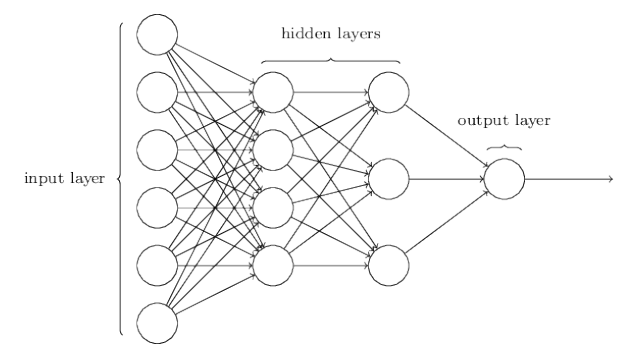
\includegraphics[width=0.65\textwidth]{figures/michael-nielsen-nn-architecture.png}
    \caption{An example of a neural network architecture~\cite{michael-nielsen-nn}}
    \label{fig:nn-example-architecture}
\end{figure}

The difference between \gls{nn} and \gls{cnn} is the among others the architectural blueprint. In \gls{cnn} neurons also have another property: the neurons are arranged in three dimensions: \textcquote{introduction-to-cnn}{the spatial dimensionality of the input(\textbf{height} and the \textbf{width}), and the \textbf{depth}}. The spatial dimensionality is the pixels, and the depth is one, since \gls{mnist} is monochrome.


%Ugly figure and not 100% visual, but it is simple
\begin{figure}[htb!]
    \centering
    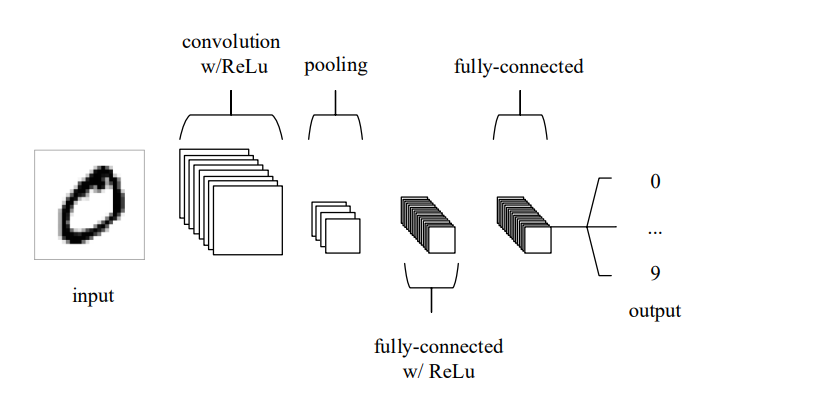
\includegraphics[width=0.8\textwidth]{figures/cnn-simple-architecture.png}
    \caption{An example of a convolutional neural network architecture~\cite{introduction-to-cnn}}
    \label{fig:simple-cnn-architecture}
\end{figure}
%Blog-like structure where CNN is depicted

\gls{cnn}'s architecture constitutes three different types of layers: convolutional layers, pooling layers, and fully-connected layers. The architecture of a \gls{cnn} can be shown in Figure \ref{fig:simple-cnn-architecture}. The convolutional layers \textcquote{introduction-to-cnn}{will determine the output of neurons of which are connected to local regions of the input}, which is also called a convolution. The pooling layers reduce the number of parameters in the previous layers. The fully-connected layers act as normal \gls{nn} layers~\cite{introduction-to-cnn}.


A convolution, as described, acts as a filter which maps the input to an output matrix $conv$ of size $n \times n$. The mapping is done by the elementwise-multiplication of the input matrix with the $conv$ matrix. The operation can be seen in Figure \ref{fig:convolution}. The manner in which such mapping is achieved is by sliding over the input matrix, from left to right, top to bottom, with a $n \times n$ matrix one pixel at a time. For each convolution operation \gls{relu} is applied to the operation, where \gls{relu} is a function which takes the maximum value between 0 and the input~\cite{google-cnn}.

\begin{figure}[htb!]
    \centering
    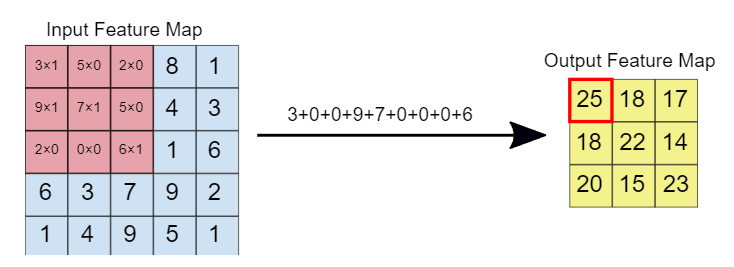
\includegraphics[width=0.7\textwidth]{figures/google-cnn-convolution-example.png}
    \caption{An example of a convolution operation~\cite{google-cnn}}
    \label{fig:convolution}
\end{figure}

In the pooling layer behaves like a convolution, but this time it filters the $conv$ matrix with a $pool$ matrix of size $n \times n$. One method which has been presented~\cite{google-cnn} is the use of max pooling; in the convolutional layer the elementwise multiplication is applied, whereas in max pooling the element with the highest number in the respective matrix is chosen~\cite{google-cnn}. Figure \ref{fig:maxpooling} is provided to show how it works. The pooling layer can be seen as a dimensionality reduction method, because it reduces the data while preserving the original features.

\begin{figure}[htb!]
    \centering
    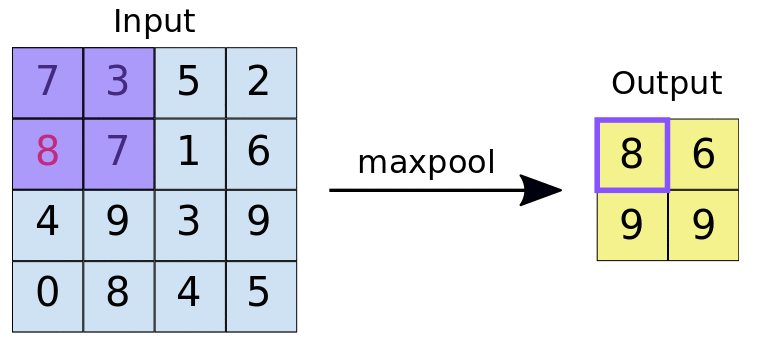
\includegraphics[width=0.5\textwidth]{figures/google-cnn-maxpooling-example.png}
    \caption{An example of a max pooling operation~\cite{google-cnn}}
    \label{fig:maxpooling}
\end{figure}

The last layer is the fully-connected layer, which is connected to all the neurons from the pooling layer. According to Keiron ~\cite{introduction-to-cnn}, the activation function \gls{relu} might be suited to be used in this layer too~\cite{lecun-mnist-database}.

\subsection{Model training}\label{subsec:model-training}
The theory deciding the cross validation methods is described in Chapter~\ref{cha:theory}.



% @book{michael-nielsen-nn,
%   title={Neural networks and deep learning},
%   author={Nielsen, Michael A},
%   volume={25},
%   year={2015},
%   publisher={Determination press San Francisco, CA, USA}
% }
% @misc{faster-svm,
%   doi = {10.48550/ARXIV.1808.06394},
  
%   url = {https://arxiv.org/abs/1808.06394},
  
%   author = {Schlag, Sebastian and Schmitt, Matthias and Schulz, Christian},
  
%   title = {Faster Support Vector Machines},
  
%   publisher = {arXiv},
  
%   year = {2018},
  
%   copyright = {arXiv.org perpetual, non-exclusive license}
% }


% @misc{introduction-to-cnn,
%   doi = {10.48550/ARXIV.1511.08458},
  
%   url = {https://arxiv.org/abs/1511.08458},
  
%   author = {O'Shea, Keiron and Nash, Ryan},
  
%   title = {An Introduction to Convolutional Neural Networks},
  
%   publisher = {arXiv},
  
%   year = {2015},
  
%   copyright = {arXiv.org perpetual, non-exclusive license}
% }


% @misc{mnist-classification-benchmark,
%     url = {https://paperswithcode.com/sota/image-classification-on-mnist},
%     title = {Image Classifcation onf MNIST},
%     year = {2022}
% }

% @misc{google-cnn,
%     organization = {Google},
%     url = {https://developers.google.com/machine-learning/practica/image-classification/convolutional-neural-networks},
%     title = {ML Practicum: Image Classification},
%     year = {2022}
% }

\section{Problem Statement}\label{sec:problem-statement}
\subsection{Audio} 
For models that predict what music is popular or what genre the music is we would like to see how big of an effect feature engineering has for the model. We would like to investigate which kind of dimensionality reduction works best considering both linear and nonlinear aproaches and what they contribute to in the model and when it is a better fit. The performance of these dimensionality reductions is evaluated based on how they affect the performance of the model and their visualisations.

\subsection{Pokemon}
For a model that clasifies Pokemon we would like to see how big of an effect feature engineering has for the model. We would also like to investigate which kind of dimensionality reduction works best and consider both linear and nonlinear aproaches and what they each contribute and when theyre correct to use. The performance of these aproaches might be evaluated based on their visualisations and how they affect model performance.

\subsection{Match data}
For models that predict the outcome of football matches we would like to see how big the effect of feature engineering has for the model. We would also like to investigate which kind of dimensionality reduction works best considering both linear and nonlinear aproaches and what they contribute to in the model and when it is a better fit. The performance of these dimensionality reductions is evaluated based on how they affect the performance of the model and their visualisations.
\chapter{Methodology}\label{cha:methodology}
Based on the problem statement in chapter \ref{cha:problem-analysis}, the following methodology is used to solve the problem.
% theoretical background in another chapter 

\section{Data collection}\label{sec:data-collection}
The data used is the \gls{mnist} database \cite{lecun-mnist-database}, which is a collection of handwritten digits. The data is split into a training set of 60,000 images and a test set of 10,000 images. The images are 28x28 pixels grayscale, and each pixel is the intensity of the pixel represented by a value between 0 and 255, where 0 is black and 255 is white. The images are labeled with the digit they represent creating 10 classes, and the labels are integers between 0 and 9.

\subsection{Data pre-preprocessing}\label{subsec:data-pre-preprocessing}
The data is normalized by dividing each pixel value by 255, so that the values are between 0 and 1. The data is then augmented by rotating the images by 90, 180 and 270 degrees, and flipping the images horizontally and vertically. This results in 10 times as much data as the original \gls{mnist} dataset.\todo{Include all the augmentations we actually use.}

\subsection{Data preprocessing}\label{subsec:data-preprocessing}
The data is then preprocessed by applying linear and non-linear dimensionality reduction techniques. The linear dimensionality reduction techniques are \gls{pca} and \gls{lda}. The non-linear dimensionality reduction techniques are \gls{kpca} and \gls{isomap}. The data is reduced to 2 dimensions, so that it can be visualized.

\section{Model training}\label{sec:model-training}
The \gls{svm} and \gls{cnn} models are then trained on both the original and the preprocessed data. The \gls{svm} model is trained using the \gls{sklearn} library, and the \gls{cnn} model is trained using the Keras library.

\subsection{Evaluation}\label{subsec:evaluation}
The models are evaluated using k-fold cross validation, and the results are averaged. The evaluation metrics are accuracy, precision, recall, f1-score, speed/run time, and memory usage. The confusion matrix covers the first of these. The speed/run time is measured by timing the training of the models, and the memory usage is measured by using the psutil library.

Lastly the models are evaluated on the test set and the results are compared to the results from the cross validation.\question{Do we want to compare our results to the results of other papers?}

\section{Pipeline}\label{sec:pipeline}

An automation pipeline is created based on the model in Figure~\ref{fig:python-pipeline-model}.


\begin{description}
    \setlength\itemsep{0em}
    \item[dataset] mnist
    \item[pre-preprocessing] normalization, data augmentation
    \item[preprocessing] linear and non linear dimensionality reduction (PCA, LDA, Kernel PCA, and ISOMAP)
    \item[models] SVM and CNN
    \item[evaluation] accuracy, precision, recall, f1-score, speed/run time, and memory usage
\end{description}


\begin{figure}[htb!]
    \centering
    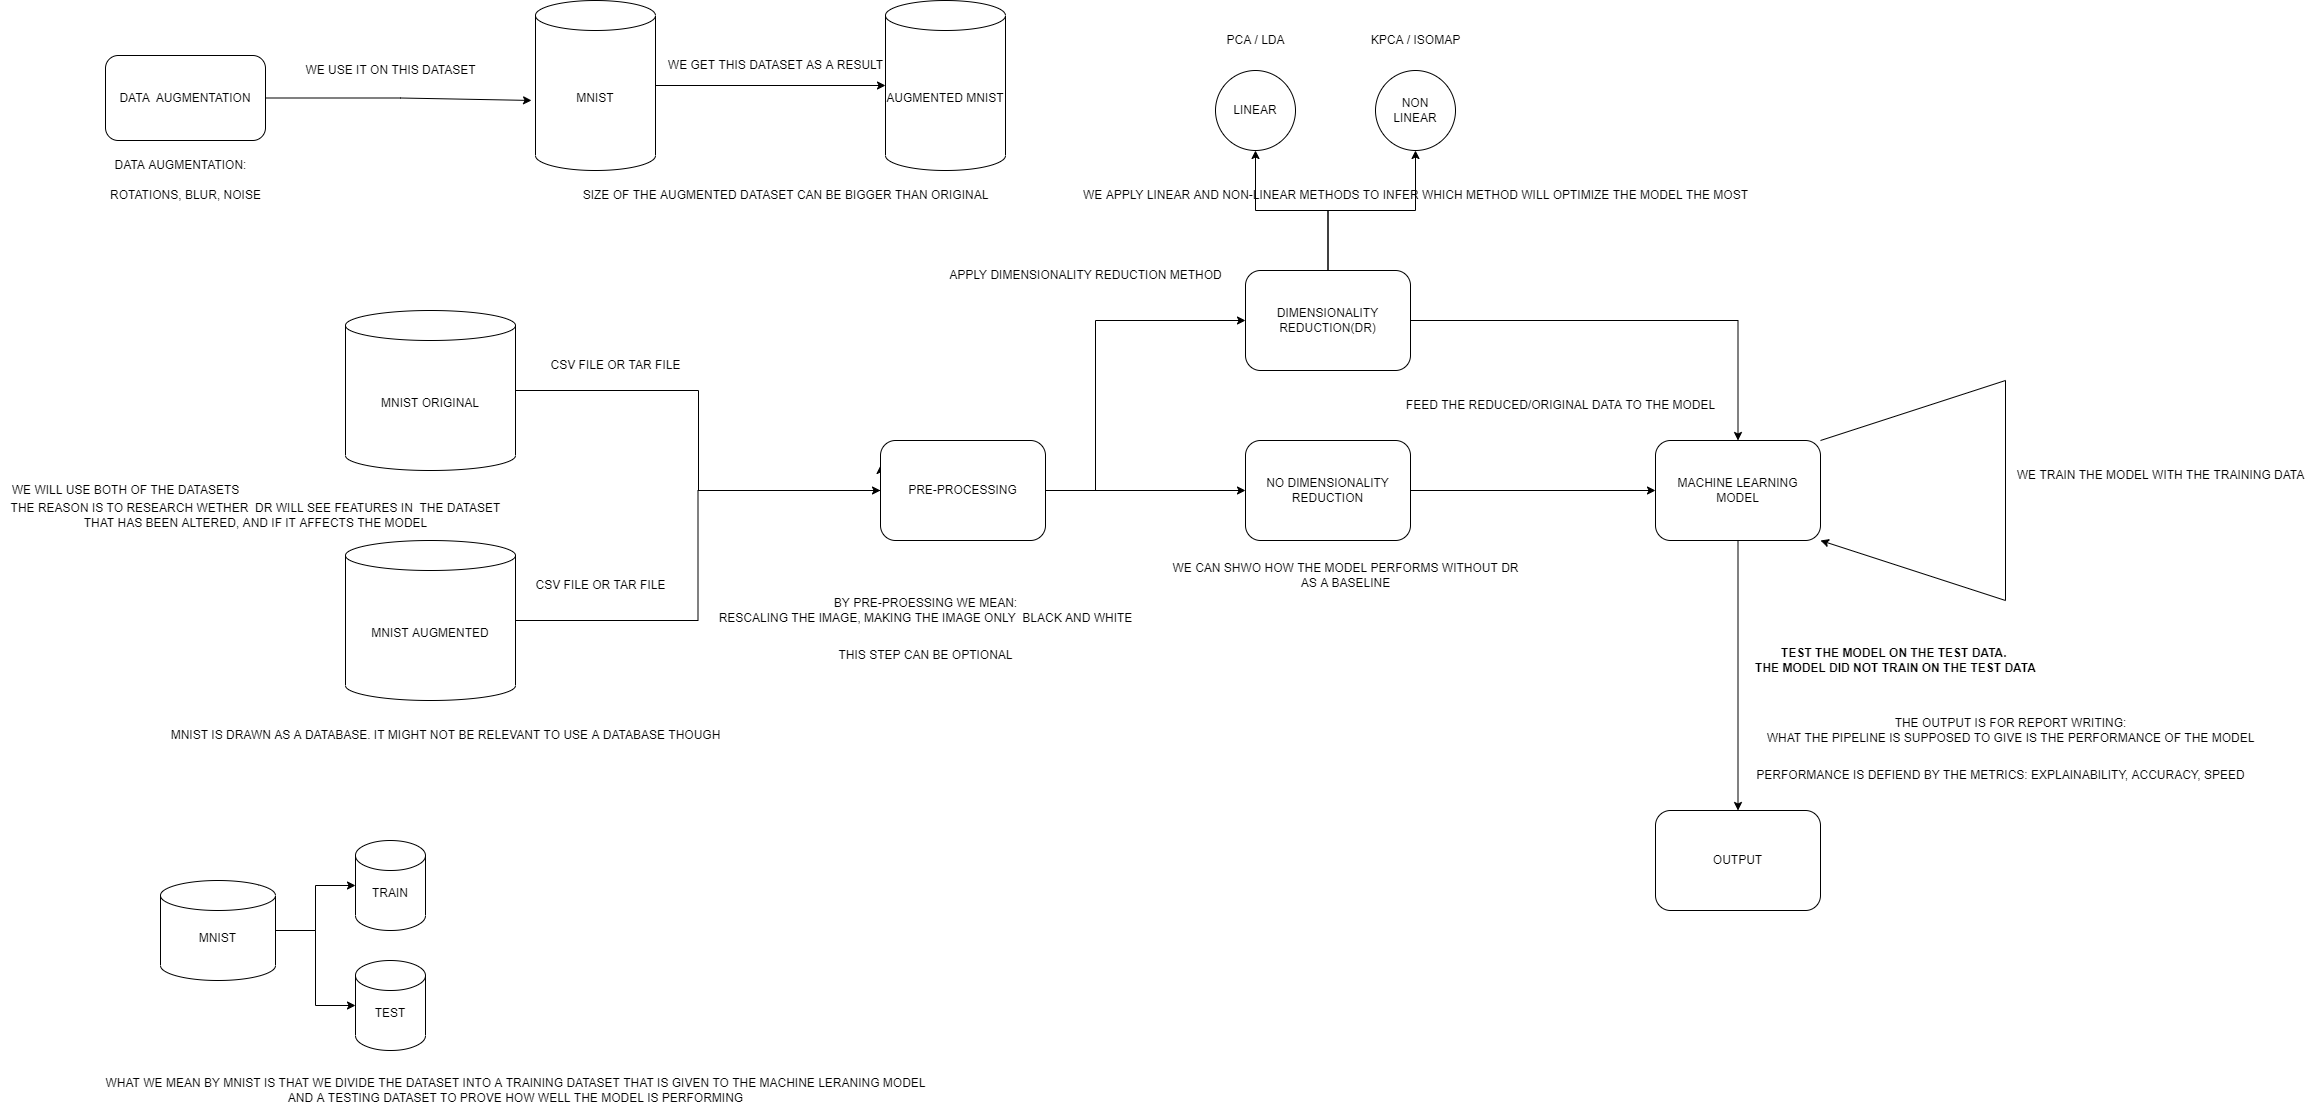
\includegraphics[width=\textwidth]{figures/pipeline-draft.png}
    \caption{Python project pipeline model.}
    \label{fig:python-pipeline-model}
\end{figure}


\urgent[inline]{write about the pipeline, and update the pipeline to include the cross validation.}

\section{Metrics}
In this project the differens dimmensionality reduction methods are evaluated based on how much it improves the metrics of our models.
The following paragraphs will go through these chosen metrics. After that the reason for the choices will be explained.

\subsection{The chosen metric}
There are 4 metrics which will be used to evaluate the FE through the model. These metrics are acurracy, precision, recall, F1-score. And there is 2 metric used to evaluate FE directly. Here the speed/computations is used to evaluate the effeciency. The other metric used is how well the dimmensionality reduction clusters the data, this will be calculated for each class as the average distance between class members divided by the average distance between all data points.

\subsection{Reason for choice of metrics}
The four model metrics were chosen because they the metric which generally describes how good the model does in infering the data. These are all essentially just variations on 
how many does the model get correct devided by diffrent parts of the confusion matrix. The last 2 metrics was chosen to show the tradeoff most models will have in the more time it takes the better results. This makes it possible to show which metric will actually be most useful in most cases since accurracy is often important only to a certain point. The second FE metric also takes into acount how well the data is clustered after aplying the FE which gives insight into how well the FE works in a vacuum and how much performance a actual model whill achiewe from data which has more defined clusters.
\chapter{Results}\label{cha:results}
Describe the results of the project.
\chapter{Discussion}\label{cha:discussion}
Discuss the results from chapter \ref{cha:results} and compare them to the problem statement in section \ref{sec:problem-statement}. Also, discuss the methodology and the theoretical background in chapter \ref{cha:methodology}. Finally, discuss the project as a whole and the process of the project.

What went well? What could have been done better? What would we do differently next time? Perhaps include thoughts on UN sustainability goals.
\chapter{Conclusion}\label{cha:conclusion}
Based on the discussion in chapter \ref{cha:discussion}, the results from chapter \ref{cha:results} and the problem statement in section \ref{sec:problem-statement}, the following conclusions can be drawn:

%backmatter
\printglossaries
\printbibliography[heading=bibintoc]\label{bib:mybiblio}

\appendix

\end{document}